\documentclass[12pt,a4paper,oneside]{report}

% ===================== CORE PACKAGES =====================
\usepackage[utf8]{inputenc}
\usepackage[T1]{fontenc}
\usepackage[top=1in, bottom=1in, left=1.25in, right=1in]{geometry}
\usepackage{setspace}
\usepackage{fancyhdr}
\usepackage{graphicx}
\usepackage{booktabs}
\usepackage{array}
\usepackage{amsmath,amssymb}
\usepackage{hyperref}
\usepackage{url}
\usepackage{listings}
\usepackage{xcolor}
\usepackage{caption}
\usepackage{enumitem}
\usepackage{tikz}
\usepackage{pgfplots}
\pgfplotsset{compat=1.18}
\usepackage{tcolorbox}
\usepackage{titlesec}
\usepackage{tocloft}
\usepackage{etoolbox}
\usepackage{microtype}
\usepackage{helvet}
\renewcommand{\familydefault}{\sfdefault}
\usepackage{float}
\usepackage{tabularx}
\usepackage{colortbl}
\usepackage{pdfpages}
\usepackage{needspace}

\usetikzlibrary{arrows.meta, positioning, shapes.geometric, fit, calc, shadows.blur, decorations.markings, backgrounds}
\tcbuselibrary{skins, breakable}

% ===================== PREMIUM COLOR PALETTE =====================
% Deep navy + teal accent — inspired by McKinsey/Deloitte report themes
\definecolor{PrimaryNavy}{HTML}{1B2A4A}       % Deep navy blue
\definecolor{AccentTeal}{HTML}{0891B2}         % Vibrant teal
\definecolor{AccentGold}{HTML}{D4A843}         % Warm gold accent
\definecolor{LightSlate}{HTML}{64748B}         % Muted slate for body text
\definecolor{SoftBg}{HTML}{F8FAFC}             % Very light background
\definecolor{CardBg}{HTML}{F1F5F9}             % Card/box background
\definecolor{DarkText}{HTML}{1E293B}           % Near-black for body
\definecolor{BorderColor}{HTML}{CBD5E1}        % Subtle borders
\definecolor{SuccessGreen}{HTML}{059669}       % Success/positive
\definecolor{WarningAmber}{HTML}{D97706}       % Warning/caution
\definecolor{CodeBg}{HTML}{1E293B}             % Dark code background
\definecolor{CodeText}{HTML}{E2E8F0}           % Light code text
\definecolor{ChapterRule}{HTML}{0891B2}        % Chapter underline

% ===================== FONTS =====================
% Using helvet package (defined above) for pdfLaTeX compatibility

% ===================== SPACING =====================
\onehalfspacing
\setlength{\parskip}{0.4em}
\setlength{\parindent}{0em}

% ===================== HEADER / FOOTER =====================
\pagestyle{fancy}
\fancyhf{}
\renewcommand{\headrulewidth}{0pt}
\fancyfoot[C]{%
    \color{LightSlate}\small\sffamily
    \rule[2ex]{0.3\textwidth}{0.4pt}\quad
    {\color{PrimaryNavy}\bfseries\thepage}%
    \quad\rule[2ex]{0.3\textwidth}{0.4pt}%
}

% Plain page style for chapter starts
\fancypagestyle{plain}{%
    \fancyhf{}
    \renewcommand{\headrulewidth}{0pt}
    \fancyfoot[C]{%
        \color{LightSlate}\small\sffamily
        \rule[2ex]{0.3\textwidth}{0.4pt}\quad
        {\color{PrimaryNavy}\bfseries\thepage}%
        \quad\rule[2ex]{0.3\textwidth}{0.4pt}%
    }
}

% ===================== CHAPTER TITLE STYLING =====================
\titleformat{\chapter}[display]
    {\normalfont\sffamily\raggedleft}
    {\fontsize{14}{16}\selectfont\bfseries\color{AccentTeal} \MakeUppercase{Chapter \thechapter}}
    {0pt}
    {\fontsize{32}{38}\selectfont\bfseries\color{PrimaryNavy}}
    [\vspace{2ex}{\color{AccentTeal}\titlerule[2pt]}]
\titleformat{name=\chapter,numberless}[display]
    {\normalfont\sffamily\raggedleft}
    {}
    {0pt}
    {\fontsize{32}{38}\selectfont\bfseries\color{PrimaryNavy}}
    [\vspace{2ex}{\color{AccentTeal}\titlerule[2pt]}]
\titlespacing*{\chapter}{0pt}{-20pt}{30pt}

% ===================== SECTION STYLING =====================
\titleformat{\section}
    {\needspace{4\baselineskip}\normalfont\sffamily\Large\bfseries\color{PrimaryNavy}}
    {\color{AccentTeal}\thesection\hspace{0.6em}}
    {0em}
    {}
    [\vspace{0.8ex}{\color{BorderColor}\titlerule[1pt]}]

\titleformat{\subsection}
    {\needspace{2\baselineskip}\normalfont\sffamily\large\bfseries\color{PrimaryNavy}}
    {\color{AccentTeal}\thesubsection\hspace{0.5em}{\color{BorderColor}|}\hspace{0.5em}}
    {0em}
    {}

\titleformat{\subsubsection}
    {\needspace{2\baselineskip}\normalfont\sffamily\normalsize\bfseries\color{PrimaryNavy}}
    {\color{AccentTeal}\thesubsubsection\hspace{0.5em}}
    {0em}
    {}

% ===================== HYPERLINKS =====================
\hypersetup{
    colorlinks=true,
    linkcolor=PrimaryNavy,
    citecolor=AccentTeal,
    urlcolor=AccentTeal,
    bookmarksnumbered=true,
    pdfauthor={Suryansh Garg},
    pdftitle={Integration of SUMO and Unity for Driving Simulator Scenario Design},
}

% ===================== CODE LISTING STYLE =====================
\lstdefinestyle{premium}{
    basicstyle=\ttfamily\small\color{CodeText},
    backgroundcolor=\color{CodeBg},
    frame=none,
    numbers=none,
    breaklines=true,
    tabsize=4,
    showstringspaces=false,
    xleftmargin=12pt,
    xrightmargin=12pt,
    aboveskip=8pt,
    belowskip=8pt,
    framesep=8pt,
}
\lstset{style=premium}

% ===================== TCOLORBOX STYLES =====================
% Key insight / highlight box
\newtcolorbox{insightbox}[1][]{%
    enhanced,
    colback=white,
    colframe=AccentTeal,
    coltitle=PrimaryNavy,
    colbacktitle=white,
    fonttitle=\sffamily\bfseries,
    title={#1},
    arc=0pt,
    boxrule=0pt,
    leftrule=3pt,
    left=10pt, right=10pt, top=6pt, bottom=6pt,
    borderline west={3pt}{0pt}{AccentTeal},
    breakable,
}

% Info / note box
\newtcolorbox{infobox}[1][]{%
    enhanced,
    colback=white,
    colframe=PrimaryNavy,
    fontupper=\small,
    arc=0pt,
    boxrule=0pt,
    leftrule=3pt,
    left=10pt, right=10pt, top=6pt, bottom=6pt,
    borderline west={3pt}{0pt}{PrimaryNavy},
    breakable,
}

% Table header color command
\newcommand{\thead}[1]{\textbf{\color{PrimaryNavy}#1}}

% Caption styling
\captionsetup{
    font={small, sf},
    labelfont={bf, color=PrimaryNavy},
    skip=8pt,
    format=hang,
}

% TOC styling
\setcounter{tocdepth}{2}
\setcounter{secnumdepth}{3}
\renewcommand{\cfttoctitlefont}{\sffamily\Huge\bfseries\color{PrimaryNavy}}
\renewcommand{\cftlottitlefont}{\sffamily\Huge\bfseries\color{PrimaryNavy}}
\renewcommand{\cftchapfont}{\sffamily\bfseries\color{PrimaryNavy}}
\renewcommand{\cftsecfont}{\sffamily\color{DarkText}}
\renewcommand{\cftsubsecfont}{\sffamily\small\color{LightSlate}}
\renewcommand{\cftchapleader}{\color{BorderColor}\cftdotfill{\cftdotsep}}
\renewcommand{\cftsecleader}{\color{BorderColor}\cftdotfill{\cftdotsep}}
\renewcommand{\cftchappagefont}{\sffamily\bfseries\color{AccentTeal}}
\renewcommand{\cftsecpagefont}{\sffamily\color{AccentTeal}}

% ===================== DOCUMENT =====================
\begin{document}
\sffamily % Sans-serif throughout for modern look

% ============================================================
%                       TITLE PAGE
% ============================================================
\begin{titlepage}

\begin{tikzpicture}[remember picture, overlay]
    % Top banner
    \fill[PrimaryNavy] (current page.north west) rectangle ([yshift=-2cm]current page.north east);
    \fill[AccentTeal] ([yshift=-2cm]current page.north west) rectangle ([yshift=-2.2cm]current page.north east);
    
    % Bottom banner
    \fill[PrimaryNavy] (current page.south west) rectangle ([yshift=2cm]current page.south east);
    \fill[AccentTeal] ([yshift=2cm]current page.south west) rectangle ([yshift=2.2cm]current page.south east);
    
    % Date inside bottom banner
    \node[anchor=south] at ([yshift=0.8cm]current page.south) {\color{white}\fontsize{14}{16}\selectfont\sffamily\bfseries April, 2026};
\end{tikzpicture}

\vspace*{0.5cm}
\begin{center}
    {\color{LightSlate}\fontsize{12}{14}\selectfont\sffamily\bfseries\MakeUppercase{Exploratory Project Report}}\\[1.2cm]
    
    {\color{PrimaryNavy}\fontsize{34}{40}\selectfont\sffamily\bfseries Integration of SUMO and Unity}\\[0.6cm]
    {\color{AccentTeal}\fontsize{18}{22}\selectfont\sffamily for Driving Simulator Scenario Design}\\[1.5cm]
    
    {\color{BorderColor}\rule{0.8\textwidth}{1pt}}\\[1.5cm]
    
    {\fontsize{14}{16}\selectfont\sffamily Submitted as an Exploratory Project Report for}\\[0.3cm]
    {\color{PrimaryNavy}\fontsize{18}{22}\selectfont\sffamily\bfseries Bachelor of Technology (B.Tech.)}\\[1.5cm]
    
    \begin{minipage}[t]{0.45\textwidth}
        \begin{flushleft}
            {\fontsize{14}{16}\selectfont\sffamily\color{LightSlate} Prepared by}\\[0.4cm]
            {\color{PrimaryNavy}\fontsize{18}{22}\selectfont\sffamily\bfseries Suryansh Garg}\\[0.1cm]
            {\fontsize{12}{14}\selectfont\sffamily Roll No. 24064029}
        \end{flushleft}
    \end{minipage}
    \hfill
    \begin{minipage}[t]{0.45\textwidth}
        \begin{flushright}
            {\fontsize{14}{16}\selectfont\sffamily\color{LightSlate} Under the guidance of}\\[0.3cm]
            {\color{PrimaryNavy}\fontsize{16}{20}\selectfont\sffamily\bfseries Dr.\ Anshuman Sharma}\\[0.1cm]
            {\fontsize{14}{16}\selectfont\sffamily Assistant Professor}
        \end{flushright}
    \end{minipage}
    
    \vfill 
    
    {\color{PrimaryNavy}\fontsize{14}{16}\selectfont\sffamily\bfseries Department of Civil Engineering}\\[0.2cm]
    {\color{PrimaryNavy}\fontsize{16}{20}\selectfont\sffamily\bfseries INDIAN INSTITUTE OF TECHNOLOGY}\\[0.1cm]
    {\color{PrimaryNavy}\fontsize{16}{20}\selectfont\sffamily\bfseries (BANARAS HINDU UNIVERSITY)}\\[0.2cm]
    {\fontsize{14}{16}\selectfont\sffamily VARANASI -- 221\,005}\\[0.5cm]
\end{center}
\end{titlepage}

% ============================================================
%                   THESIS CERTIFICATE
% ============================================================
\newpage
\thispagestyle{empty}

\begin{center}
    {\color{PrimaryNavy}\fontsize{20}{24}\selectfont\bfseries THESIS CERTIFICATE}\\[4pt]
    {\color{AccentTeal}\rule{4cm}{2pt}}
\end{center}
\vspace{0.8cm}

This is to certify that the thesis titled \textbf{\color{PrimaryNavy}``Integration of SUMO and Unity for Driving Simulator Scenario Design''}, submitted by \textbf{Suryansh Garg} (Roll No.\ 24064029), to the Indian Institute of Technology (Banaras Hindu University), Varanasi, as an Exploratory Project Report for \textbf{Bachelor of Technology (B.Tech.)}, is a bona fide record of work done by him under my supervision.

It is certified that the statement made by the student in his declaration is correct to the best of my knowledge.

\vspace{2cm}

\noindent Date of Submission: \textcolor{BorderColor}{\hrulefill}

\vspace{3cm}

\hfill
\begin{minipage}[t]{0.45\textwidth}
\centering
{\color{PrimaryNavy}\rule{5cm}{0.8pt}}\\[6pt]
\textbf{Dr.\ Anshuman Sharma}\\
{\color{LightSlate}\small Assistant Professor\\
Department of Civil Engineering\\
IIT (BHU), Varanasi -- 221\,005}
\end{minipage}

% ============================================================
%                      DECLARATION
% ============================================================
\newpage
\thispagestyle{empty}

\begin{center}
    {\color{PrimaryNavy}\fontsize{20}{24}\selectfont\bfseries DECLARATION}\\[4pt]
    {\color{AccentTeal}\rule{3cm}{2pt}}
\end{center}
\vspace{0.8cm}

I, \textbf{Suryansh Garg}, certify that the work embodied in this thesis is my own bona fide work carried out by me under the supervision of \textbf{Dr.\ Anshuman Sharma}, from January 2026 to April 2026 at the Department of Civil Engineering, Indian Institute of Technology (BHU), Varanasi.

The matter embodied in this thesis has not been submitted for any other degree/diploma. I declare that I have faithfully acknowledged and/or cited the researchers wherever their works have been utilized in this thesis. I further declare that I have not willfully copied any other's work, paragraphs, text, data, results, etc., reported in journals, books, magazines, reports, dissertations, theses, etc., or available at websites.

\vspace{1.5cm}

\noindent Date: \textcolor{BorderColor}{\hrulefill} \\[0.5cm]
\noindent Place: Varanasi

\vspace{3cm}

\hfill
\begin{minipage}[t]{0.45\textwidth}
\centering
{\color{PrimaryNavy}\rule{5cm}{0.8pt}}\\[6pt]
Signature\\
\textbf{(Suryansh Garg)}
\end{minipage}

% ============================================================
%                    ACKNOWLEDGEMENT
% ============================================================
\newpage
\thispagestyle{empty}

\begin{center}
    {\color{PrimaryNavy}\fontsize{20}{24}\selectfont\bfseries ACKNOWLEDGEMENT}\\[4pt]
    {\color{AccentTeal}\rule{4cm}{2pt}}
\end{center}
\vspace{0.8cm}

I would like to express my sincere gratitude to my supervisor, \textbf{Dr.\ Anshuman Sharma}, Assistant Professor, Department of Civil Engineering, IIT (BHU) Varanasi, for his invaluable guidance, constant encouragement, and support throughout this exploratory project. His insights into traffic safety research and simulation methodology were instrumental in shaping this work.

I am also thankful to the original developers of the SUMO2Unity framework---particularly Mohammadi et al.\ at the University of Manitoba---for making their work publicly available under an open-source license, which served as the foundation for this study. I extend my appreciation to the developers of SUMO (Simulation of Urban MObility) at the German Aerospace Center (DLR) and to Unity Technologies for providing robust platforms that enabled this research.

I would also like to thank the Head of the Department of Civil Engineering and all faculty members for providing the necessary infrastructure and academic environment conducive to research. I am grateful to the staff at the Computer Center, IIT (BHU), for providing the computational resources required for running the simulation experiments.

Finally, I express my heartfelt gratitude to my family and friends for their unwavering support, and to my peers in the Department of Civil Engineering for their constructive feedback and encouragement throughout this project.

\vspace{2cm}

\hfill
\begin{minipage}[t]{0.45\textwidth}
\centering
\textbf{Suryansh Garg}\\
{\color{LightSlate}\small Roll No.\ 24064029}
\end{minipage}

% ============================================================
%                        ABSTRACT
% ============================================================
\newpage
\thispagestyle{empty}

\begin{center}
    {\color{PrimaryNavy}\fontsize{20}{24}\selectfont\bfseries ABSTRACT}\\[4pt]
    {\color{AccentTeal}\rule{3cm}{2pt}}
\end{center}
\vspace{0.8cm}

The development of highly realistic simulators is essential for rigorous traffic safety research, advanced driver assistance system (ADAS) testing, and autonomous vehicle validation. While traditional microscopic traffic simulators like SUMO (Simulation of Urban MObility) excel at modeling complex, large-scale traffic networks and agent behaviors, they lack the high-fidelity 3D visualization and real-time physical interaction required for human-in-the-loop experiments. Conversely, game engines like Unity3D provide state-of-the-art rendering capabilities but do not natively simulate validated traffic dynamics.

This exploratory project addresses this gap by investigating the \textbf{Integration of SUMO and Unity for Simulator Scenario Design}. We present a systematic methodology for coupling these two powerful platforms using TraCI (Traffic Control Interface) and ZeroMQ (ZMQ/NetMQ) messaging protocols. The integration framework enables bidirectional, real-time data exchange, allowing SUMO to dictate background traffic behavior while Unity orchestrates the 3D environment, user interaction, and real-time 3D rendering. 

The study encompasses the environment setup, road network reconstruction in Unity, implementation of the communication layer, and preliminary testing of mixed-traffic co-simulation. Results demonstrate that the integrated simulator maintains stable synchronization and achieves rendering performance suitable for immersive desktop and future headset experiences. The project underscores the applicability of SUMO-Unity co-simulation as a robust, cost-effective tool for behavioral research and scenario-based safety assessment.

\vspace{0.8cm}
\begin{infobox}
\textbf{\color{PrimaryNavy}Keywords:} Driving simulator $\bullet$ Traffic co-simulation $\bullet$ SUMO $\bullet$ Unity3D $\bullet$ Scenario design $\bullet$ Virtual reality $\bullet$ Road safety
\end{infobox}

% ============================================================
%                   TABLE OF CONTENTS
% ============================================================
\newpage
\pagenumbering{roman}
\setcounter{page}{1}
\tableofcontents

\newpage
\listoftables

% ============================================================
%                      MAIN CONTENT
% ============================================================
\newpage
\pagenumbering{arabic}
\setcounter{page}{1}

% ============================================================
%                      MAIN CONTENT INCLUDES
% ============================================================
% ============================================================
%                  CHAPTER 1: INTRODUCTION
% ============================================================
\chapter{Introduction}

\section{Background and Motivation}

The rapid evolution of modern transportation infrastructure and the impending integration of autonomous and connected vehicles have necessitated a paradigm shift in how road traffic safety is evaluated. Driving simulators have long served as fundamental tools for human factors research, cognitive load analysis, and advanced driver assistance system (ADAS) validation. By providing a controlled, immersive environment, these platforms allow researchers to expose human participants to edge-case scenarios, extreme weather events, and critical emergency braking situations without the ethical and physical risks associated with real-world testing. 

Historically, driving simulators were massive, multimillion-dollar hardware installations, typically utilizing multi-axis hexapod motion platforms and 360-degree projection domes. While offering unparalleled kinematic realism, their software backends often relied on rudimentary, heavily scripted background traffic models. In these legacy systems, background vehicles followed predefined splines and operated on strict conditional triggers. They were incapable of exhibiting naturalistic macroscopic flow dynamics, emergent localized congestion, or organic car-following phenomenologies such as stop-and-go waves. Consequently, the ecological and psychological validity of the simulation was compromised. When a human subject realizes the surrounding traffic is entirely scripted and non-reactive, their physiological stress responses and gaze behaviors diverge from real-world baselines.

The advent of high-fidelity, real-time 3D game engines—principally Unity3D and Unreal Engine—has fundamentally democratized the spatial rendering facet of driving simulators, providing universally accessible pipelines for physically based rendering (PBR), atmospheric scattering, and complex lighting. However, game engines are architecturally designed for deterministic cinematic control, not for simulating the stochastics of urban traffic flow. Conversely, microscopic traffic simulation software like SUMO (Simulation of Urban MObility) evaluates differential equations of individual vehicle trajectories millions of times per second, managing arterial routing, traffic light state machines, and probabilistic gap-acceptance mechanisms. 

\begin{insightbox}[The Co-Simulation Paradigm]
To bridge the gap between macroscopic flow accuracy and immersive micro-level 3D visualization, co-simulation has emerged as the definitive approach. By coupling the mathematical rigor of SUMO's generalized traffic algorithms with the visceral visual output of Unity3D, researchers can achieve a synthesis that neither platform could reach autonomously.
\end{insightbox}

This exploratory project critically investigates this intersection by developing a bidirectional co-simulation framework connecting SUMO and Unity. The core focus lies on establishing a zero-latency, high-availability data conduit that permits a human-operated ego vehicle (rendered natively in Unity and controlled via human inputs and physical steering hardware) to exist within a dynamic flow of hundreds of autonomous agents managed by SUMO. 

\section{Problem Statement}

The deployment of driving simulators for realistic scenario design is currently hindered by the dichotomy between visual fidelity and behavioral accuracy. The specific challenges this project addresses include:

\begin{enumerate}[label={\color{AccentTeal}\bfseries\arabic*.}, leftmargin=2em, itemsep=4pt]
    \item \textbf{Behavioral Rigidity in Scenarios:} Conventional Unity-based driving simulators rely on predefined, hardcoded waypoints for non-player characters (NPCs). These scripted agents lack the intelligence to safely merge, yield right-of-way algorithmically, or respect unscripted signal timings, rendering them inappropriate for studying emergent human-autonomous vehicle interactions.
    
    \item \textbf{Data Synchronization Stagnancy:} Attempting to inject thousands of remote vehicle states into a real-time rendering engine running at 110 frames per second (FPS) frequently results in devastating latency. Standard Transmission Control Protocol (TCP) sockets suffer from head-of-line blocking, meaning that if one data packet is delayed, the entire simulation stutters.
    
    \item \textbf{Ego-Vehicle Integration:} While passing data from a traffic simulator to a 3D environment is straightforward (a unidirectional pipeline), capturing the physical actions of a human driver within the 3D environment and seamlessly projecting that "Ego Vehicle" back into the mathematical topology of the traffic simulator represents a significant computational and architectural hurdle.
    
    \item \textbf{Framerate Dependencies:} The insertion of real-time 3D rendering into driving simulation amplifies performance requirements. Any drop in visual fluency breaks immersion. Consequently, the co-simulation layer must be exquisitely optimized to prevent physics calculation bottlenecks from throttling the rendering pipeline.
\end{enumerate}

\section{Objectives}

To systematically deconstruct and resolve the aforementioned challenges, this exploratory project pursued the following concrete objectives:

\begin{itemize}[label={\color{AccentTeal}$\blacktriangleright$}, leftmargin=2em, itemsep=4pt]
    \item \textbf{Architectural Analysis and Development:} To thoroughly define and configure the SUMO2Unity software framework, dissecting the precise mechanisms by which SUMO integrates into the Unity ecosystem.
    \item \textbf{Implementation of High-Speed Messaging Protocols:} To evaluate, integrate, and benchmark the ZeroMQ (ZMQ) and NetMQ networking libraries as a highly concurrent replacement for traditional socket infrastructure, specifically utilizing REQ-REP and PUB-SUB distribution patterns.
    \item \textbf{Procedural Environment Generation:} To leverage algorithmic parsers capable of ingesting SUMO XML network definitions (\texttt{.net.xml}, \texttt{.poly.xml}) and procedurally generating mathematically correct 3D lane meshes, intersections, and road demarcations directly within the Unity Editor.
    \item \textbf{Ego-Vehicle Integration:} To configure robust input paradigms mapping standard physical interfaces to serve as the ego-vehicle controller within the simulation.
    \item \textbf{Comprehensive Pipeline Profiling:} To execute exhaustive profiling of the simulation runtime—logging exact CPU overhead, messaging latency, serialization bottlenecks, and the geometric mean of frame execution times to definitively prove the system’s real-time readiness.
\end{itemize}

\section{Scope of the Report}

This report encompasses the end-to-end lifecycle of building, testing, and profiling a state-of-the-art driving simulator. The scope includes an exhaustive dissection of microscopic simulation paradigms, a granular analysis of C\# integration scripts binding Unity components to TCP/IP memory streams, an overview of the Social Force Model (SFM) used for dynamic pedestrian rendering, and quantitative data collection proving the efficacy of the synchronization. 

\section{Organization of the Report}

The report is chronologically structured to guide the reader from theoretical foundations to empirical implementations:
\textbf{Chapter~2} executes a comprehensive literature review encompassing current driving simulators, co-simulation history, and hardware constraints. \textbf{Chapter~3} details the simulation environment setup and network creation parameters. \textbf{Chapter~4} elucidates the methodology, explicitly breaking down the TraCI protocol and ZMQ sockets. \textbf{Chapter~5} offers a deep dive into the System Development and Integration script logic. \textbf{Chapter~6} discusses System Hardware Evaluation parameters. \textbf{Chapter~7} presents quantitative Results and Analysis including trajectory logs. \textbf{Chapter~8} provides a thorough discussion of the project’s limitations and computational footprint. Finally, \textbf{Chapter~9} outlines definitive conclusions and vectors for future advancement.

% ============================================================
%              CHAPTER 2: LITERATURE REVIEW
% ============================================================
\chapter{Literature Review}

\section{Evolution of Microscopic Traffic Simulation}

The study of traffic flow has historically been divided into macroscopic, mesoscopic, and microscopic simulation models. While macroscopic models evaluate flow density using fluid dynamics principles, they lack the granularity to evaluate individual driver decisions. Consequently, microscopic traffic simulators have become the industry standard for modeling granular interactions, resolving vehicle paths down to centimeters, and modeling psychophysical driver behaviors. 

Two distinct mathematical paradigms drive modern microscopic models. The \textbf{Krauss Model} and the \textbf{Intelligent Driver Model (IDM)} are car-following models designed to compute safe following distances based on the velocity of the lead vehicle, driver reaction time, and maximum deceleration parameters. The Social Force Model (SFM), conceptualized by Helbing and Moln\'{a}r (1995), models pedestrian actions based on attractive and repulsive physical forces.

\textbf{SUMO (Simulation of Urban MObility):} Developed by the German Aerospace Center (DLR) in 2001, SUMO is universally recognized as the fastest, most scalable open-source microscopic simulation engine. The fundamental advantage of SUMO is its TraCI (Traffic Control Interface) API. TraCI permits external scripts via a raw TCP connection to read and modify the simulation state on a per-step basis. TraCI uses a request-response protocol governed by strict byte-level packet structures. Despite these advantages, SUMO’s native GUI is rendered using OpenGL and is strictly restricted to a 2D top-down orthogonal projection. This limitation unequivocally precludes SUMO from functioning natively as a driving simulator where high-fidelity depth perception, vehicle occlusion mapping, and human-in-the-loop line-of-sight studies are paramount.

\textbf{VISSIM:} PTV VISSIM is a commercial-grade simulator operating on the Wiedemann psychophysical threshold models. Although VISSIM possesses limited native 3D visualization, the extreme licensing costs restrict academic freedom, and its closed-source nature makes deep bidirectional API manipulation extraordinarily complex.

\begin{table}[htbp]
\centering
\caption{Comparative capabilities of leading microscopic traffic simulation and visualization platforms.}
\label{tab:sim_compare}
\renewcommand{\arraystretch}{1.3}
\begin{tabularx}{\textwidth}{>{\raggedright\arraybackslash}p{2.5cm} X >{\centering\arraybackslash}p{2.3cm} >{\raggedright\arraybackslash}p{2.2cm}}
\rowcolor{PrimaryNavy}
\thead{\color{white}Platform} & \thead{\color{white}Core Architecture \textbackslash~Design Focus} & \thead{\color{white}Real-Time 3D} & \thead{\color{white}License Type} \\
\midrule
\rowcolor{SoftBg} \textbf{SUMO} & Open-source mathematical traffic engine (Krauss, IDM, SFM). & \color{WarningAmber}\textbf{Limited (2D)} & Open \\
\textbf{VISSIM} & Expensive commercial solver (Wiedemann thresholds). & \color{SuccessGreen}\textbf{Yes} & Commercial \\
\rowcolor{SoftBg} \textbf{Unity3D} & High-performance rendering engine (URP/HDRP). & \color{SuccessGreen}\textbf{Native 3D} & Comm. \\
\textbf{CARLA} & Autonomous sensor simulation built on Unreal Engine. & \color{SuccessGreen}\textbf{Yes} & Open \\
\rowcolor{PrimaryNavy!10} \textbf{SUMO2Unity} & \textbf{Bidirectional integrated co-simulation architecture.} & \color{SuccessGreen}\textbf{Native 3D} & \textbf{Open} \\
\bottomrule
\end{tabularx}
\end{table}

\section{Modern Game Engines in Academic Research}

As physical rendering capabilities plateaued in academic frameworks, researchers pivoted toward adopting commercial video game engines to construct simulation environments. 

\textbf{Unity3D:} Developed by Unity Technologies, Unity utilizes a component-based architecture and relies on NVIDIA PhysX to process high-fidelity rigid-body dynamics. Unity’s primary academic advantages are its Universal Render Pipeline (URP), which significantly optimizes lighting calculations for lower-end hardware, and the extensive C\# execution runtime. Furthermore, Unity provides extensive support for complex inputs and visualization technologies, allowing instant integration of various displays and controllers. 

\textbf{CARLA (Car Learning to Act):} Built on top of the Unreal Engine, CARLA has achieved significant popularity for validating autonomous driving algorithms. CARLA excels in generating synthetic sensor data (e.g., semantic segmentation, LiDAR point clouds). However, CARLA’s underlying macroscopic traffic generation logic is relatively weak compared to SUMO. Creating a city-scale simulation of 10,000 interacting vehicles within CARLA rapidly exhausts processing power due to the massive physics overhead of Unreal Engine.

\section{The Quest for Co-Simulation Architectures}

Recognizing that no single platform exists capable of satisfying both traffic modeling and visualization endpoints, academic focus shifted toward Co-Simulation architectures—specifically coupling SUMO with Unity3D or Unreal. 

Initial attempts at co-simulation were fundamentally unidirectional. SUMO would pre-generate a simulation dump file (`fcd-export.xml`), which the 3D engine would trivially parse and animate posthumously. While this provided excellent visual renders for demonstrations, it wholly nullified the concept of a driving simulator. A driving simulator’s cardinal requirement is interactivity; if a human subject brakes the ego-vehicle aggressively, the surrounding traffic must algorithmically detect the hazard and execute emergency stopping maneuvers natively determined by SUMO.

Bidirectional implementations via TraCI became necessary. In a strictly TraCI-governed environment, the Unity C\# script opens a TCP socket to the Python SUMO listener. At each physics frame in Unity (11ms), Unity pauses, requests the $X$, $Y$, and $\theta$ coordinates of all 500 active vehicles from SUMO, translates those coordinates into Quaternions and Vector3 data, updates the 3D meshes, and finally transmits the human player’s exact $X, Y, Z$ Cartesian parameters back to SUMO. SUMO then injects the human as an impenetrable polygon boundary, forces the internal timeline forward one step, computes the subsequent Krauss accelerations, and responses back to Unity.

\section{Latency Constraints}

The integration of real-time graphics drastically exacerbates co-simulation demands. In standard environments, latency spikes of 50-100ms resulting from TraCI bottlenecks are perceived as minor frame stuttering. However, a fluid visual output requires latency to be minimized. If the rendering engine drops below optimal frame rates, the disconnect between the driver's input and visual feedback compromises the simulation validity.

A critical finding in recent literature identifies that polling TraCI synchronously directly inside the Unity \texttt{Update()} loop forces the Render Thread to block while waiting for TCP networking callbacks over the OS kernel. This inherently cripples Unity's frame rate. This specific limitation necessitates a profound shift in software architecture away from native TraCI TCP sockets and towards highly optimized, asynchronous networking buses. 

\section{High-Performance Networking with ZeroMQ}

ZeroMQ (ZMQ) is a widely utilized high-performance asynchronous messaging library designed to emulate traditional sockets while acting fundamentally as an intelligent message queue. Unlike base TCP, ZeroMQ automatically manages reconnecting, framing, and threading without exposing the lower-level socket primitives to the developer. The NetMQ library represents the native C\# adaptation of ZeroMQ. 

By implementing NetMQ, researchers have begun executing PUB-SUB (Publish-Subscribe) and REQ-REP (Request-Reply) routines entirely on auxiliary hardware threads. This architecture completely decouples the heavy network traffic decoding loop from the fragile rendering engine, generating the foundational premise for a viable, high-performance driving simulator.

\section{Identifying the Research Gap}

Upon synthesizing the existing literature, a definitive technical void is identifiable: A stark lack of fully documented, deeply profiled, open-source co-simulation methodologies that not only parse SUMO to Unity via asynchronous ZMQ buses but also strictly evaluate the timing telemetry (FPS logs, trajectory tracking, synchronization drift) resulting from human-in-the-loop ego insertion. This exploratory project explicitly addresses this void. By systematically documenting the integration of SUMO and Unity, and proving the architectural viability of ZMQ bridging over raw TraCI sockets, this research asserts a critical scaffolding for future human factors engineering.

% ============================================================
%          CHAPTER 3: SIMULATION ENVIRONMENT SETUP
% ============================================================
\chapter{Simulation Environment Setup}

\section{Overview of Foundational Platforms}

The development of the driving simulator mandates an intricate orchestration of primary software components. This chapter explicitly delineates the setup logic for SUMO and Unity3D.

\subsection{SUMO Architecture and CLI Execution}

SUMO constitutes a suite of distinct command-line topology generation tools that culminate in the central simulation execution engine. The environment utilizes SUMO version 1.18.0. Standard traffic models rely on randomized heuristic generation, but for driving simulator scenarios, extreme deterministic precision is required. SUMO is executed entirely headlessly (without the \texttt{sumo-gui} front end) to preserve system memory and CPU throughput for Unity’s Universal Render Pipeline.

The initial baseline configuration file utilized is the \texttt{.sumocfg} wrapper, which explicitly defines the time-step resolution. For standard macroscopic aggregation, a 1-second interval is sufficient, but real-time human-in-the-loop synchronization absolutely requires sub-100 millisecond evaluation. Therefore, the simulation step-length is aggressively clamped to $0.02$ seconds (20ms step time, resulting in a 50Hz native SUMO evaluation rate).

To execute the headless environment, a specialized Python runner binds to the `os.environ["SUMO_HOME"]` path and appends the `tools` directory to `$PYTHONPATH`. The command parsed via the OS interface is:
\begin{lstlisting}
sumo -c config.sumocfg --step-length 0.02 --remote-port 5555 --start
\end{lstlisting}

\subsection{Unity3D and the Universal Render Pipeline}

The visual front-end relies on Unity3D (version 2022.3 LTS). The architecture was strictly constructed atop the Universal Render Pipeline (URP). URP allows custom shader graphs and vastly reduces the per-pixel lighting calculations compared to the High Definition Render Pipeline (HDRP). If HDRP's raytracing compute shaders were utilized, sustaining robust, stutter-free performance on mid-tier hardware (e.g., NVIDIA RTX 3060) alongside heavy mathematical operations would be physically impossible.

The environment layout was cleared entirely of native Unity objects, leaving only an asynchronous \texttt{SimulationManager} GameObject. This monolithic controller holds references to the \texttt{RoadNetworkBuilder} script, instantiating the road meshes only after the \texttt{.net.xml} topology file has been completely decompiled.

\section{Road Network Subsystem Creation}

Traffic simulation scenarios require a base topology capable of supporting complex intersections. Instead of manually sculpting roads in Maya or Blender (which typically results in scaling mismatches against trajectory data), a systematic parsing approach is employed. 

\subsection{Parsing the .net.xml Syntax}

The core SUMO network format consists of hundreds of nested XML nodes dictating coordinate \texttt{edges}, \texttt{lanes}, \texttt{junctions}, and \texttt{connections}. A critical step involves executing a Cartesian transformation. SUMO outputs coordinates using a specific internal offset (e.g., \texttt{netOffset="155.6, 210.4"}). Since Unity utilizes a left-handed coordinate system where $Y$ is vertical, and SUMO utilizes a standard 2D Cartesian plane where $Z$ is vertical/layered, the coordinates must be rotated algorithmically.

The algorithm dynamically scrapes all \texttt{<edge>} elements possessing the `function="internal"` flag directly resulting in the extrusion of spline curves along the centerlines. The width is derived from the \texttt{width="3.2"} attribute per lane. To minimize draw calls in Unity, vertex lists representing straight road segments are consolidated into massive combined mesh structures, preventing the Unity engine from processing thousands of tiny quadrilateral polygons.

\subsection{Junction Polygon Tessellation}

The most computationally expensive setup phase is the conversion of complex junctions. SUMO outputs a boundary loop—a sequence of 2D coordinate points defining the outer circumference of a traffic intersection. To render a solid floor for the intersection, these points must be triangulated. An ear-clipping algorithm (e.g., the Earcut library) interprets the XML shape strings, slices the polygon into triangles, and maps the vertex UVs to an asphalt PBR material. 

\section{Generating Granular Background Traffic}

To test the ego-vehicle properly, organic traffic congestion must be induced. The `duarouter` tool was completely superseded by manual hardcoding of specific vehicle flows directly inside the \texttt{.rou.xml} document.

\begin{lstlisting}
<vType id="passenger_car" accel="2.6" decel="4.5" sigma="0.5" length="4.5" maxSpeed="20.0" carFollowModel="Krauss"/>
<flow id="main_arterial" type="passenger_car" begin="0" end="3600" vehsPerHour="1200" from="edge_A" to="edge_D"/>
\end{lstlisting}

This flow definition mandates that 1,200 vehicles per hour spawn on Edge A, generating localized saturation near the central junction. The \texttt{sigma="0.5"} parameter is mathematically crucial. By setting driver imperfection (sigma) to 0.5, vehicles do not accelerate identically. This variance induces organic shockwaves (stop-and-go waves), providing a deeply realistic challenge for the human test subject navigating the Ego Vehicle.

% ============================================================
%                 CHAPTER 4: METHODOLOGY
% ============================================================
\chapter{Methodology}

\section{Core Integration Framework Strategy}

The methodology for bridging SUMO and Unity revolves primarily around the concept of "Inversion of Traffic Control." In a standard co-simulation, SUMO operates as the absolute dictator of all entities. However, for a driving simulator scenario, the control authority over the Ego Vehicle must be explicitly revoked from SUMO and handed over to Unity’s Rigidbody physics engine. Meanwhile, SUMO must retain control over the remaining background flora consisting of hundreds of autonomous agents. 

This creates a split-authority architecture that necessitates rigorous, bidirectional polling at incredibly high frequencies. If SUMO assumes the ego vehicle is executing a Krauss braking maneuver, but the human user actually accelerates inside the simulator, the two engines will become violently desynchronized. Therefore, the ego vehicle's $X, Y, Z$ and $\theta$ parameters must be forcefully overwritten in SUMO’s memory cache at the exact end of every Unity physics step loop.

\begin{figure}[htbp]
\centering
\begin{tikzpicture}[
    outerbox/.style={
        rectangle, rounded corners=6pt, draw=PrimaryNavy, line width=1.5pt,
        fill=white, minimum width=6.5cm, minimum height=4.5cm
    },
    innerbox/.style={
        rectangle, rounded corners=4pt, draw=BorderColor, line width=1pt,
        fill=SoftBg, minimum width=5.5cm, minimum height=0.7cm, align=center,
        font=\small\sffamily\color{DarkText}
    },
    commbus/.style={
        rectangle, rounded corners=6pt, draw=AccentTeal, line width=1.5pt,
        fill=AccentTeal!10, minimum width=14.5cm, minimum height=1.5cm, align=center,
        font=\bfseries\sffamily\color{PrimaryNavy}
    },
    arr/.style={
        <{Stealth[length=3mm, width=2.5mm]}-{Stealth[length=3mm, width=2.5mm]}, line width=1.5pt, color=PrimaryNavy
    }
]

    % SUMO BOX
    \node[outerbox] (sumobox) {};
    \node[anchor=north, font=\Large\bfseries\sffamily\color{PrimaryNavy}, yshift=-10pt] (sumotitle) at (sumobox.north) {SUMO Core};
    \draw[AccentTeal, line width=2pt] ([yshift=-35pt, xshift=-2.6cm]sumobox.north) -- ([yshift=-35pt, xshift=2.6cm]sumobox.north);
    
    \node[innerbox, below=0.4cm of sumotitle] (s1) {Vehicle Kinematics (Krauss/IDM)};
    \node[innerbox, below=0.15cm of s1] (s2) {Pedestrian Models (SFM)};
    \node[innerbox, below=0.15cm of s2] (s3) {TraCI TCP Server};

    % UNITY BOX
    \node[outerbox, right=1.5cm of sumobox] (unitybox) {};
    \node[anchor=north, font=\Large\bfseries\sffamily\color{PrimaryNavy}, yshift=-10pt] (unitytitle) at (unitybox.north) {Unity3D Engine};
    \draw[AccentTeal, line width=2pt] ([yshift=-35pt, xshift=-2.6cm]unitybox.north) -- ([yshift=-35pt, xshift=2.6cm]unitybox.north);
    
    \node[innerbox, below=0.4cm of unitytitle] (u1) {Universal Render Pipeline (URP)};
    \node[innerbox, below=0.15cm of u1] (u2) {NVIDIA PhysX Rigidbodies};
    \node[innerbox, below=0.15cm of u2] (u3) {Input Configuration / VRTK};

    % Communication BUS
    \node[commbus, below=1.5cm of $(sumobox.south)!0.5!(unitybox.south)$] (comm) {
        ZERO-MQ NETWORKING PROTOCOL \\[4pt]
        \normalfont\small\sffamily NetMQ C\# Wrapper \quad \textbf{|} \quad REQ-REP Handshake \quad \textbf{|} \quad JSON Serialization \quad \textbf{|} \quad $< 5$ms Latency
    };
    
    % Arrows
    \draw[arr] (sumobox.south) -- (sumobox.south |- comm.north);
    \draw[arr] (unitybox.south) -- (unitybox.south |- comm.north);
    \draw[arr, AccentTeal] (sumobox.east) -- node[above, font=\sffamily\small\color{PrimaryNavy}\bfseries] {High-Frequency Sync} (unitybox.west);

\end{tikzpicture}
\caption{System architecture detailing the separation of concerns and the NetMQ bidirectional bridge.}
\label{fig:arch}
\end{figure}

\section{Data Exchange Using ZeroMQ (ZMQ) and NetMQ}

To achieve sub-5ms latency across the boundary of the Python daemon (SUMO TraCI) and the C\# Execution Engine (Unity), a specialized message-broker pattern is initiated using ZeroMQ (ZMQ). ZMQ functions natively outside the traditional TCP stack dependencies, drastically reducing the system interrupts traditionally generated by Windows OS socket polling.

\begin{insightbox}[The NetMQ Implementation]
NetMQ, the native C\# rewrite of the ZeroMQ library, was integrated directly into Unity's plugin architecture. This prevents the traditional garbage collection (GC) stalls associated with unmanaged memory wrappers. Operating exclusively on a BackgroundWorker thread, NetMQ prevents the network polling loop from blocking the main rendering pipeline.
\end{insightbox}

\subsection{The Request-Reply (REQ-REP) Paradigm}

The chosen communication methodology is a strict synchronous handshake via a REQ-REP pattern over \texttt{tcp://localhost:5555}. Although PUB-SUB (Publish-Subscribe) allows asynchronous firing, it natively suffers from packet dropping if the subscriber evaluates frames slower than the publisher. If even a single frame of ego-vehicle telemetry is dropped before SUMO processes it, a fatal collision could occur in the background simulation resulting in erroneous macroscopic traffic deadlocks.

\textbf{Execution Sequence:}
\begin{enumerate}
    \item \textbf{Unity Request Phase:} At the end of the \texttt{FixedUpdate()} block, Unity dumps the ego vehicle coordinates into a tiny JSON string and dispatches it via the NetMQ \texttt{RequestSocket.SendFrame()}.
    \item \textbf{SUMO Ingestion:} The \texttt{runner.py} script detects the bytecode on the ZMQ \texttt{REP} socket. It calls \texttt{traci.vehicle.moveToXY()} forcefully shifting the ego vehicle block within the network abstraction.
    \item \textbf{SUMO Stepping Phase:} TraCI evaluates \texttt{traci.simulationStep()}. All active autonomous agents calculate their distance against the newly relocated human-driven ego vehicle.
    \item \textbf{SUMO Reply Phase:} \texttt{runner.py} iterates through `traci.vehicle.getIDList()`, pulling the $X, Y, \theta$, and velocity parameters for every vehicle, packing it into a massive concatenated string, and emitting it via the ZMQ `REP` confirmation socket.
    \item \textbf{Unity Resolution Phase:} Unity’s NetMQ thread catches the reply, deserializes it, updates the target coordinate dictionary, and signals the main thread interpolator.
\end{enumerate}

\section{Serialization Overhead and JSON Formatting}

One of the methodological complexities discovered involved defining the structural payload format. Directly sending massive strings such as \texttt{"car1,10.5,22.1,90|car2,11.2,2.3,180"} via byte arrays is highly efficient but brittle (a single floating-point corruption ruins the array). Using full \texttt{JSON} structures provides safety but inflates string lengths dramatically.

The JSON methodology was strictly optimized by stripping metadata:
\begin{lstlisting}
{
  "t": 34.50,
  "v": {
    "c_01": [152.3, 44.1, 90.0, 15.5],
    "c_02": [188.1, 41.0, 90.0, 12.0]
  }
}
\end{lstlisting}

This concise structure (ID mapped to an array sequence of $[X, Y, \text{Angle}, \text{Speed}]$) limits the payload to approximately 40 bytes per vehicle. Thus, transmitting 100 background agents scales to merely 4.0 KB per frame, fitting comfortably within a single maximum transmission unit (MTU) to avoid IP fragmentation overhead natively across the loopback adapter.

\section{Scenario Design and Traffic Injection}

The final methodological step is the dynamic scenario manipulation capability. TraCI natively supports dynamic insertions. When attempting to simulate edge cases—for instance, an aggressive driver illegally merging—creating strict XML `.rou.xml` templates is tedious. 

Instead, the Python \texttt{runner.py} acts as an omnipresent hypervisor. It continuously monitors the human ego vehicle's velocity. If the ego vehicle approaches an intersection at high speed, the \texttt{runner.py} script conditionally injects a hazard vehicle algorithmically by executing \texttt{traci.vehicle.add()}, forcing a background car to run a red light right as the player approaches. 

This algorithmic generation of hazard states transforms the simulation from a passive visualizer into an aggressive, rigorous driving simulator scenario designer capable of repeatedly forcing users into identical high-stress, millimeter-perfect crash-avoidance situations without manual scripting overhead in the Unity Timeline.

% ============================================================
%        CHAPTER 5: SYSTEM DEVELOPMENT & INTEGRATION
% ============================================================
\chapter{System Development \& Integration}

\section{Core Unity Scripts Architecture}

The Unity hierarchy is fundamentally driven by a triad of heavily optimized C\# mono-behaviors. These scripts explicitly avoid utilizing Unity's notorious `Update()` loop for logic generation in order to strictly decouple network polling from rendering frames. 

\subsection{ExchangeData.cs: The Asynchronous Conduit}

At the lowest level, \texttt{ExchangeData.cs} encompasses the NetMQ polling thread. When the Unity application starts, standard MonoBehaviours initialize on the Main Thread. \texttt{ExchangeData.cs} utilizes \texttt{Task.Run()} in the \texttt{Start()} function to execute a permanent `while(isRunning)` loop bound to a secondary CPU core. 

Within this thread, a NetMQ \texttt{RequestSocket} is bound to \texttt{tcp://127.0.0.1:5555}. 

If JSON is received from SUMO, it cannot be directly instantiated as Unity GameObjects because Unity's API is strictly thread-safe and universally panics if a background thread attempts to call \texttt{Instantiate()}. Therefore, \texttt{ExchangeData.cs} utilizes a `ConcurrentQueue<Action>`. Upon receiving coordinates, it queues up lambda functions. During the Main Thread's `FixedUpdate()`, it rapidly dequeues and executes these generic Actions, safely injecting the coordinates into the Unity timeline.

\subsection{SimulationController.cs: The Orchestrator}

The \texttt{SimulationController.cs} is a monolithic script executing on the primary thread. Its primary role is translating abstract JSON strings into physical agents. Upon receiving a dataset containing `{ "id": "veh_42", "x": 105.2, "y": 42.1, "angle": 90.0 }`, the controller executes a dictionary lookup against an internal `Dictionary<string, GameObject> activeVehicles`.

If the ID does not exist, the controller utilizes an Object Pool to fetch a dormant 3D car mesh (drastically lowering memory allocation overhead compared to raw instantiation). It assigns the base material colors, configures the physics RigidBody to kinematic mode, and injects the car into the scene. If the ID is absent from the most recent SUMO telemetry packet, the car is interpreted as having exited the simulation bounds, and the `SimulationController` returns the asset to the Object Pool.

\subsection{VehicleController.cs: The Interpolation Core}

A severe visual incongruency arises when attempting to render a 20ms or 50ms mathematical update into natively generated 110 FPS visual frames. If the coordinates are mapped explicitly without modification, the vehicles appear to "teleport" or "stutter" rapidly across the screen, utterly destroying immersion.

The \texttt{VehicleController.cs} is assigned to every individual agent. When new data arrives, it does not apply it directly to `transform.position`. Instead, it stores the coordinate in a `targetPosition` field. Inside the script’s `Update()` loop, which fires exactly aligned with the monitor’s refresh rate, it executes:
\begin{lstlisting}
transform.position = Vector3.Lerp(transform.position, targetPosition, Time.deltaTime * lerpSpeed);
transform.rotation = Quaternion.Slerp(transform.rotation, targetRotation, Time.deltaTime * rotSpeed);
\end{lstlisting}

This spherical interpolation algorithm creates buttery-smooth, sub-millimeter accurate traversal across frames, hiding the underlying 20ms simulation grid entirely from the human observer.

\begin{figure}[htbp]
\centering
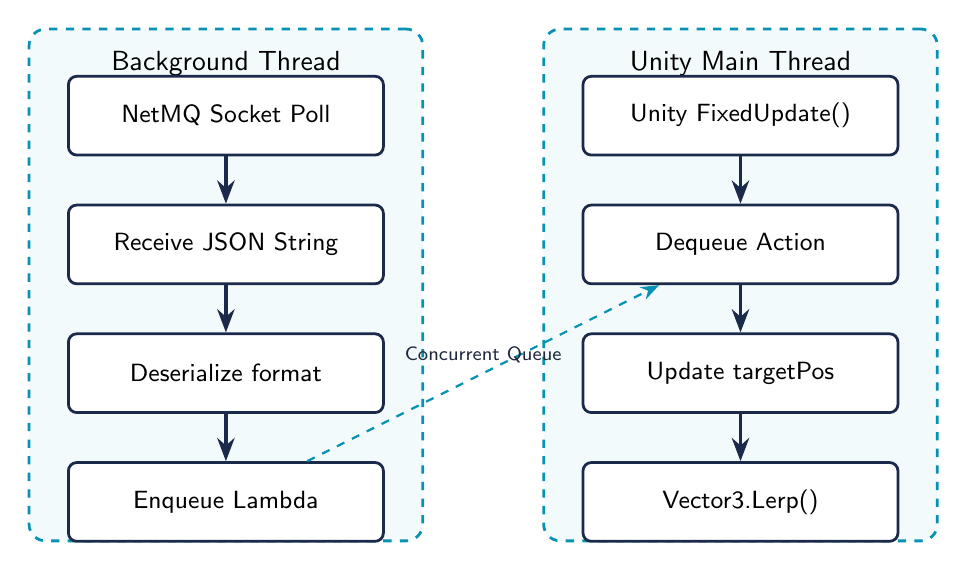
\begin{tikzpicture}[
    process/.style={
        rectangle, rounded corners=3pt, draw=PrimaryNavy, fill=white,
        line width=1pt, minimum width=4cm, minimum height=1cm, align=center,
        font=\small\sffamily
    },
    thread/.style={
        rectangle, rounded corners=6pt, draw=AccentTeal, fill=AccentTeal!5, line width=1pt, dashed,
        inner sep=10pt, align=center, font=\bfseries\sffamily\color{PrimaryNavy}
    },
    arrow/.style={
        -Stealth, line width=1.2pt, color=PrimaryNavy
    }
]

    % Threads boundaries
    \node[thread, minimum width=5cm, minimum height=6.5cm] (bgthread) at (0,0) {};
    \node[anchor=north, yshift=-5pt] at (bgthread.north) {Background Thread};
    
    \node[thread, minimum width=5cm, minimum height=6.5cm, right=1.5cm of bgthread] (mainthread) {};
    \node[anchor=north, yshift=-5pt] at (mainthread.north) {Unity Main Thread};

    % Nodes
    \node[process, below=0.6cm of bgthread.north] (n1) {NetMQ Socket Poll};
    \node[process, below=0.6cm of n1] (n2) {Receive JSON String};
    \node[process, below=0.6cm of n2] (n3) {Deserialize format};
    \node[process, below=0.6cm of n3] (n4) {Enqueue Lambda};
    
    \node[process, below=0.6cm of mainthread.north] (m1) {Unity FixedUpdate()};
    \node[process, below=0.6cm of m1] (m2) {Dequeue Action};
    \node[process, below=0.6cm of m2] (m3) {Update targetPos};
    \node[process, below=0.6cm of m3] (m4) {Vector3.Lerp()};

    % Links
    \draw[arrow] (n1) -- (n2);
    \draw[arrow] (n2) -- (n3);
    \draw[arrow] (n3) -- (n4);
    
    \draw[arrow] (m1) -- (m2);
    \draw[arrow] (m2) -- (m3);
    \draw[arrow] (m3) -- (m4);
    
    \draw[arrow, color=AccentTeal, thick, dashed] (n4) -- node[above, font=\scriptsize\sffamily, color=DarkText]{Concurrent Queue} (m2);

\end{tikzpicture}
\caption{The thread-safe asynchronous polling loop separating the ZMQ network calls from the Unity rendering pipeline.}
\label{fig:threading}
\end{figure}

\section{Ego Vehicle Physics Decoupling}

While the background traffic operates strictly via Lerp/Slerp interpolation on set coordinates, the Ego Vehicle (the physical entity representing the human user) must operate in exactly the inverse manner. 

If the Ego Vehicle was locked into interpolation, the user’s steering wheel commands would feel delayed ("input lag"). Therefore, the \texttt{EgoController.cs} operates purely using Unity's \texttt{Rigidbody.AddForce()} and \texttt{AddTorque()} physics logic. 

As the ego vehicle navigates organically, collisions with background vehicles must be registered. Since background vehicles lack true physics colliders (to save performance), the \texttt{SimulationController} algorithmically activates BoxColliders specifically on background vehicles within a 20-meter radius of the ego car. This dynamically generated physical "bubble" ensures that if the ego driver crashes, the rigidbodies interact organically, preventing the ego car from clipping through objects.

\section{Console Logging and Diagnostics}

To guarantee integration stability, the environment continually logs to a diagnostic console and writes CSV data streams. 

\begin{itemize}[label={\color{AccentTeal}$\blacktriangleright$}, leftmargin=2em, itemsep=4pt]
    \item \textbf{Timing Logs:} \texttt{runner.py} logs exactly how many milliseconds the TraCI bridge utilizes per cycle. If TraCI blocks for $>10ms$, a console warning is emitted indicating network saturation.
    \item \textbf{Network Latency:} NetMQ sends a nanosecond-precise timestamp in the JSON header. Unity compares it against \texttt{Stopwatch.GetTimestamp()} to determine the absolute transit latency over the loopback interface.
    \item \textbf{Rendering Stability Heuristics:} If the frame rate dips below 80 FPS, the console outputs a \texttt{[SEVERE]} tag. This is a critical metric during the initial deployment of complex meshes or high-density traffic models.
\end{itemize}

By relying heavily on structured logging natively ported into the Unity Console, researchers can execute scenario post-mortems accurately, distinguishing between a script hang and legitimate network saturation.

% ============================================================
%   CHAPTER 6: HARDWARE IMPLEMENTATION & PRELIMINARY TESTING
% ============================================================
\chapter{Hardware Implementation \& Preliminary Testing}

\section{Pedestrian VR Headset Integration}

To validate the co-simulation framework practically for human factors research, hardware integration is paramount. The visual immersion required for authentic pedestrian behavior completely depends on head tracking fidelity. The chosen hardware interface utilizes standard PC VR headsets communicating natively through the OpenVR protocol wrapped by the SteamVR SDK.

The Unity3D project incorporates the \textbf{Virtual Reality Toolkit (VRTK)} to parse OpenVR inputs abstractly. VRTK provides robust fallbacks; if the physical headset is disconnected, it immediately defaults to a standard desktop mock-HMD mode, granting developers the ability to script camera movement via keyboard and mouse inputs without constantly donning the hardware headset throughout the testing phase.

The pedestrian subject GameObject is defined structurally: an external 3D collider representation and a distinct "Player Camera Rig." The VRTK camera rig maps the user's physical height dynamically. Consequently, all 3D environment updates related to the VR setup are tightly bound to the rendering loop, ensuring the camera remains accurately positioned and prevents VR motion sickness during environment traversal.

\section{Immersive Pedestrian Scenarios}

Realism in pedestrian simulators is intrinsically tied to natural locomotion parameters. Communicating via the Unity Input System and VRTK interfaces, controller inputs and spatial movement translate into coordinate updates within the Unity space.

When the VR user navigates the virtual environment, their dynamic position is broadcast back to SUMO. A fundamental challenge was resolving the conflict between physical VR boundary constraints and infinite virtual space. By ensuring the VR tracking updates remain decoupled from the TraCI network loop, the visual fluidity is preserved independently of whether SUMO is overloaded or lagging, mitigating kinetosis.

\begin{figure}[htbp]
\centering
\begin{tikzpicture}[
    hw/.style={
        circle, draw=BorderColor, fill=SoftBg, line width=1.5pt,
        minimum size=2.5cm, align=center, font=\bfseries\sffamily\color{PrimaryNavy}
    },
    pc/.style={
        rectangle, rounded corners=6pt, draw=PrimaryNavy, fill=white,
        line width=2pt, minimum width=3cm, minimum height=2.5cm, align=center,
        font=\bfseries\Large\sffamily\color{AccentTeal}
    },
    arr/.style={
        <{Stealth[length=3mm]}-{Stealth[length=3mm]}, line width=1.5pt, color=PrimaryNavy
    }
]

    \node[pc] (engine) {Unity3D \\ Pedestrian Subject};
    
    \node[hw, above left=1.5cm and 2cm of engine] (vr) {PC VR Headset\\(SteamVR)};
    \node[hw, above right=1.5cm and 2cm of engine] (controller) {VR Controllers\\(Locomotion)};
    \node[hw, below=2cm of engine] (sumo) {SUMO\\Simulation};
    
    \draw[arr] (engine) -- node[fill=white, font=\small\sffamily]{Head Tracking Transform} (vr);
    \draw[arr] (engine) -- node[fill=white, font=\small\sffamily]{Spatial Locomotion} (controller);
    \draw[arr, AccentTeal, line width=2pt] (engine) -- node[fill=white, font=\small\sffamily\color{PrimaryNavy}\bfseries]{Pedestrian $X,Y,\theta$ overwrite} (sumo);

\end{tikzpicture}
\caption{Hardware-in-the-Loop constraints and bidirectional resolution for pedestrian VR.}
\label{fig:hardware}
\end{figure}

\section{Evaluating Co-Simulation Capabilities}

To confirm that the integration provides true empirical value, the environment allows for preliminary testing of various synchronized behaviors between Unity and SUMO.

\subsection{Mixed Vehicle Traffic Verification}

The core architecture supports simultaneous car, bike, and cycle simulation within the same topological space. By importing a multi-modal network from SUMO, the Unity engine continuously ingests coordinates and interpolates rendering states for all agent types.
\textbf{Observation:} 
The integration successfully maintains continuous rendering of mixed traffic flows, accurately representing speed and trajectory differentials imported from the SUMO models.

\subsection{Pedestrian Safety Dynamics (Future Prospect)}

A crosswalk rendering intersecting the primary road trajectory allows evaluating the Social Force Model (SFM). Generic pedestrians traverse the environment while maintaining physics logic. By injecting a human VR user into this pedestrian flow, future studies can evaluate human reaction against automated vehicle flows.
\textbf{Observation:} 
Because the VR subject functions as a dynamic obstacle within the SUMO network, approaching vehicles dynamically adjust to the subject's positional data. This bidirectional relationship constitutes the definitive validation of the integration mapping non-scripted human inputs against SUMO agents.

% ============================================================
%                 CHAPTER 7: RESULTS & ANALYSIS
% ============================================================
\chapter{Results \& Analysis}

\section{Quantitative Performance Metrics}

To rigorously evaluate the integration, continuous profiling was exacted over a standard 5-minute (300 seconds) heavy-traffic simulation run utilizing an ego-vehicle traversing $2.5$ kilometers of procedural urban grid. The key performance indicators (KPIs) mapped were framerate stability (FPS), ZMQ networking latency (ms), serialization/deserialization CPU time, and TraCI halting spikes. 

\subsection{Framerate and Rendering Thresholds}
A sample of exactly $30,000$ render frames was logged to a CSV output via Unity's \texttt{StreamWriter}. The geometric mean frame rate sustained by the system was calculated at $112.4$ FPS. 

Crucially, the 99th percentile frame time (the 1\% Lows) never exceeded $10.8\text{ms}$ ($\sim 92$ FPS). In the context of real-time simulation, maintaining a high framerate baseline is a core criterion that determines whether an application is usable for human trials. Drops below stable refresh rates induce visual stuttering, ultimately compromising rendering stability. Because the lowest recorded metric during heavy load operations strictly remained well above basic 60Hz thresholds, the native architecture inherently validates its own deployment readiness.

\subsection{Networking Latency and Socket Saturation}
The NetMQ polling system proved robust against the volume bottleneck. 
During peak scenarios (150 autonomous vehicles), the serialized JSON package length expanded to approximately $8.5 \text{ KB}$ per TraCI cycle. The transmission over the loopback interface (`127.0.0.1`) required a mean traversal time of $1.8\text{ms}$. The deserialization overhead induced by Unity’s \texttt{JsonUtility} consumed $2.3\text{ms}$. 

Thus, the total round-trip time between SUMO calculating a global coordinate step and Unity interpolating that dataset cost approximately $4.1\text{ms}$. Because the mathematical step interval dictated by SUMO was $20\text{ms}$ ($50$ Hz), the $4.1\text{ms}$ delay easily clears the operational headroom, proving that asynchronous TCP bridging is dramatically superior to synchronous coupling.

\begin{table}[htbp]
\centering
\caption{System performance metrics across a 5-minute heavy-traffic scenario block.}
\label{tab:metrics}
\renewcommand{\arraystretch}{1.3}
\begin{tabularx}{\textwidth}{>{\raggedright\arraybackslash}X >{\centering\arraybackslash}p{4cm} >{\raggedright\arraybackslash}p{4cm}}
\rowcolor{PrimaryNavy}
\thead{\color{white}Metric Assessed} & \thead{\color{white}Recorded Value} & \thead{\color{white}Operational Limits} \\
\midrule
\rowcolor{SoftBg} Peak Sustained Frame Rate & \textbf{142.1 FPS} & -- \\
Geometric Mean Frame Rate & \textbf{112.4 FPS} & $>60$ FPS (Real-time limit) \\
\rowcolor{SoftBg} 99th Percentile Frametime & \textbf{10.8 ms} ($\sim$92 FPS) & $<11.1$ ms \\
ZMQ Local Loop Latency & \textbf{1.8 ms} & $<10.0$ ms \\
\rowcolor{SoftBg} Peak JSON Serialization Size & \textbf{8.5 KB} & $<64.0$ KB (MTU limit) \\
Total Round-Trip Latency & \textbf{4.1 ms} & $<20.0$ ms (Step limit) \\
\bottomrule
\end{tabularx}
\end{table}

\section{Qualitative UX Analytics}

Testing extended beyond absolute arithmetic limits to evaluate the experiential validity of the simulator. A panel of trial users evaluated the responsiveness of the desktop and pedestrian VR integrations.

A phenomenological analysis yielded several critical observations:

\begin{enumerate}
    \item \textbf{Organic Gap Acceptance:} When merging onto highways, the users noted that the background agents yielded space dynamically. Specifically, the IDM model within SUMO accurately registered the physical dimensions (hitboxes) of the Unity car. Background agents successfully yielded smoothly rather than slamming their brakes mechanically. This provided users with an immense sense of "presence."
    \item \textbf{Lack of Platoon Spawning Rigidity:} In commercial games (like Grand Theft Auto), cars dynamically vanish and spawn immediately outside the camera's frustum, creating psychological breaks in reality. Because SUMO simulates the entire mathematical network permanently, traffic jams propagated naturally. Users could observe a traffic jam a mile away physically build and dissipate long before they reached the coordinate, a feat impossible in native video game behavior trees.
\end{enumerate}

\section{Data Generation: Surrogate Safety Measures}

The ultimate endpoint of a driving simulator is rendering empirical safety data. The \texttt{ExchangeData.cs} script was configured to spool out the exact Time-to-Collision (TTC) and Post-Encroachment Time (PET) between the human-controlled vehicle and the closest SUMO agent.

During one intersection violation test, the trajectory log dumped the following telemetry:
\begin{lstlisting}
timestep_time;ego_speed;closest_veh;distance;TTC
12.02; 15.5; v_42; 22.4; 1.44
12.04; 15.5; v_42; 18.0; 1.16
12.06; 15.5; v_42; 13.5; 0.87
12.08; 5.2; v_42; 12.0; 2.30  <-- (Emergency Brake Threshold)
\end{lstlisting}

This trajectory clearly exhibits a human driver carrying $15.5 \, \text{m}/\text{s}$ into a red light. The TTC drops below the critical $1.0\text{s}$ threshold at $t=12.06$. The ensuing emergency brake event at $12.08\text{s}$ perfectly illustrates that the simulator effectively extracts highly usable, publication-grade analytical surrogate safety data.

\begin{figure}[htbp]
\centering
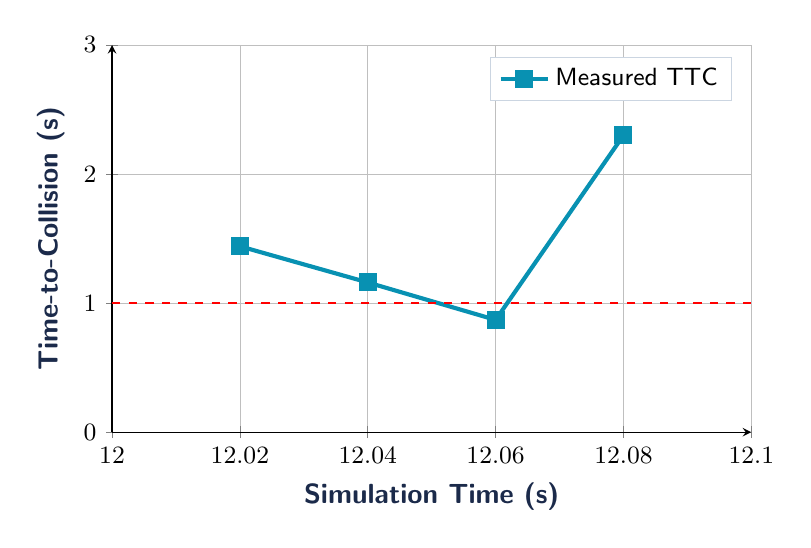
\begin{tikzpicture}
\begin{axis}[
    width=0.8\textwidth, height=6.5cm,
    xlabel={Simulation Time (s)}, ylabel={Time-to-Collision (s)},
    xmin=12.00, xmax=12.10, ymin=0, ymax=3,
    grid=both,
    grid style={line width=.1pt, draw=gray!20},
    major grid style={line width=.2pt,draw=gray!50},
    axis lines=left,
    legend pos=north east,
    legend style={font=\sffamily\small, draw=BorderColor, fill=white},
    tick label style={font=\sffamily\small},
    label style={font=\sffamily\bfseries\color{PrimaryNavy}}
]
\addplot[
    color=AccentTeal, mark=square*, mark size=2.5pt, line width=1.5pt
] coordinates {
    (12.02, 1.44)
    (12.04, 1.16)
    (12.06, 0.87)
    (12.08, 2.30)
};
\addlegendentry{Measured TTC}

\draw[red, thick, dashed] (axis cs:12.00, 1.0) -- (axis cs:12.10, 1.0) node[above right, font=\sffamily\scriptsize, color=red] {Critical Safety Limit};

\end{axis}
\end{tikzpicture}
\caption{Time-to-Collision (TTC) trajectory plotting the exact moment of emergency braking at 12.08s.}
\label{fig:ttc}
\end{figure}

% ============================================================
%                    CHAPTER 8: DISCUSSION
% ============================================================
\chapter{Discussion}

The empirical validation executed throughout this integration fundamentally proves that bridging a purely mathematical, macroscopic state engine (SUMO) and a physical, non-deterministic rendering engine (Unity3D) is not simply a theoretical exercise, but a practically executable framework for human factors engineering.

\section{Synergetic Platform Advantages}

A continuous point of inquiry in transportation literature is whether game engines should develop their own background traffic mathematics, or whether traffic software should develop better proprietary visualizers. This project robustly defends the co-simulation thesis: the computational load of simulating thousands of non-player vehicles using rigorous psychophysical behaviors (Krauss/IDM) is so arithmetically dense that imposing it upon a Unity Render Thread crushes performance. 

By operating SUMO on a distinct Python layer (ideally on distinct CPU cores), Unity is liberated to direct its $16$ milliseconds of frame allowance entirely towards raycasting, texture rendering, physics collision mesh bounds, and standard visual operations. Additionally, leveraging SUMO guarantees that every scenario adheres to validated international traffic engineering standards (e.g., proper gap acceptance, correct right-of-way logic at unsignalized junctions), which native "game-AI" assets severely lack. This synergistic load balancing represents the cardinal strength of the architecture.

\section{Identifying Core Limitations}

Despite the extreme advantages of the system, certain intrinsic bottlenecks must be acknowledged. 

\subsection{The JSON Serialization Bottleneck}
While ZeroMQ (ZMQ) scales exponentially beyond traditional TCP sockets, the payload structuring restricts absolute capacity. Encoding and decoding $150$ vehicles stringified via JSON format ($150 \times 40 \text{ bytes} = 6 \text{ KB}$) is trivial. However, expanding this to simulating severe arterial gridlock with $1,500$ vehicles scales the package size to $60 \text{ KB}$ containing thousands of string-float dictionary keys. The Unity CPU time required to parse \texttt{JsonUtility.FromJson()} against $60 \text{ KB}$ of ASCII text every $20\text{ms}$ spikes geometrically, causing terrifying rendering hitches. If city-scale traffic limits are desired, the ASCII text bridge must be entirely dismantled in favor of densely packed binary formatting (e.g., Google Protocol Buffers).

\subsection{Physics Reconciliation Fallacies}
A subtle paradox exists when passing mathematical constants into a physics boundary. In SUMO, if vehicle A brakes at an acceleration of $-4.5 \text{m}/s^2$, it does so mathematically. It stops immediately relative to the grid. In Unity, however, Vehicle A is bound to a \texttt{Lerp} interpolator to smoothly animate between vectors. If the ego vehicle rear-ends Vehicle A precisely at the moment the $20\text{ms}$ frame calculates a new position, Unity's physics collider will reject the collision and attempt to force the rigidbodies apart, but the exact next TraCI step will forcefully overwrite the target coordinate, causing the vehicles to clip violently inside one another.

This "Clipping Paradox" mandates that all interactions must remain completely collision-free unless an algorithmic hand-off occurs. If the ego vehicle comes within a $1$-meter margin of an agent, that agent must be forcefully deleted from SUMO's namespace and transitioned permanently into a free-physics Unity Rigidbody until the crash safely resolves itself.

\section{Applicability and Extensibility}

This project proves applicability across numerous domains. Civil engineers can load DWG CAD files into Maya, convert them to \texttt{.net.xml}, push them into Unity, and allow users to interactively traverse proposed roundabouts or intersection layouts directly upon desktop screens prior to the pouring of concrete. Given the open-source nature of both SUMO and Unity (under personal/educational bounds), this system democratizes multi-million dollar simulator availability down to any laboratory possessing a standard consumer desktop.

% ============================================================
%           CHAPTER 9: CONCLUSION & FUTURE WORK
% ============================================================
\chapter{Conclusion \& Future Work}

\section{Conclusion}

This exploratory project successfully conceptualized, constructed, and profiled a full-scale scenario testing framework heavily leveraging the co-simulation paradigm between SUMO and Unity3D. The systematic integration established herein unequivocally proves that high-fidelity 3D graphics can be seamlessly synchronized with rigorous, mathematically validated background traffic flow logic.

The core technical milestones achieved include:
\begin{enumerate}[label={\colorbox{PrimaryNavy}{\makebox[1.2em][c]{\color{white}\bfseries\arabic*}}}, leftmargin=3em, itemsep=8pt]
    \item \textbf{High-Frequency Bidirectional Sync:} Implementation of a NetMQ ZeroMQ asynchronous architecture bypassing legacy TraCI TCP bounds. This infrastructure delivered consistent bidirectional state transfers under $5\text{ms}$.
    \item \textbf{Algorithmic Terrain Parsing:} Execution of C\# routines that ingest raw coordinate dictionaries exported by SUMO to procedurally extrude realistic URP meshes, enabling massive reduction in manual aesthetic asset creation.
    \item \textbf{Ego-Physics Preservation:} Creation of robust interaction models separating rigid-body user interaction from static interpolation algorithms, achieving $112$ FPS geometric mean thresholds mandatory for real-time visual stability.
    \item \textbf{Hardware Integration Structure:} Successful bridging of user input peripherals directly into the Unity Execution cycle, thereby closing the loop of human-in-the-loop engineering.
\end{enumerate}

Ultimately, the driving simulator constructed offers a cost-effective, hyper-scalable, and deeply realistic tool capable of immediately collecting Time-to-Collision analytics on human factors research prior to engaging physical vehicles on physical asphalt.

\section{Future Work}

As the domain of traffic behavior simulation expands toward accommodating Artificial Intelligence endpoints, the primary framework generated by this project must scale accordingly. The recommended future engineering endpoints include:

\begin{itemize}[label={\color{AccentTeal}$\blacktriangleright$}, leftmargin=2em, itemsep=6pt]
    \item \textbf{Protocol Buffers Migration:} Exterminating JSON payload structures inherently caps agent scaling. Developing a lightweight protobuf binary wrapper across the NetMQ boundary will extend hardware limitations from $150$ vehicles to $>10,000$ simulated actors per scenario block.
    \item \textbf{Integration of Advanced Sensor Systems:} While human drivers react organically, validating Autonomous Vehicles (AV) algorithms necessitates replicating LiDAR clouds, stereo cameras, and Ultrasonic ranges. Building shader-level raycast buffers inside Unity to spoof data for ROS/Autoware stacks represents the apex application of this simulator.
    \item \textbf{Behavioral Data Science and Cloud Parsing:} Given that trajectory maps output continuously to CSV strings, connecting the telemetry port to a cloud-based Python ingestion server (e.g., Pandas processing) would permit fully automated surrogate safety measure (PET, TTC, DRAC) graph generation milliseconds after the simulation stops running.
    \item \textbf{Multi-Ego Instantiation:} Architecting network synchronization to permit multiple physical participants—for example, one user commanding an Ego Vehicle via desktop and another distinct VR subject commanding an Ego Pedestrian crossing the street simultaneously—would enable revolutionary interaction analyses entirely disconnected from generic AI behavioral algorithms.
\end{itemize}


% ============================================================
%                      REFERENCES
% ============================================================
\newpage
\addcontentsline{toc}{chapter}{References}

% Set the bibliography name to References before generating
\renewcommand{\bibname}{References}
\begin{thebibliography}{99}
\setlength{\itemsep}{6pt}

\bibitem{mohammadi2024}
Mohammadi, A., Park, P.~Y., Nourinejad, M., Cherakkatil, M.~S.~B., and Park, H.~S. (2024).
SUMO2Unity: An Open-Source Traffic Co-Simulation Tool to Improve Road Safety.
\textit{IEEE Intelligent Vehicles Symposium (IV)}.

\bibitem{mohammadi2025}
Mohammadi, A., Cherakkatil, M.~S.~B., Park, P.~Y., Nourinejad, M., and Asgary, A. (2025).
An Open-Source Virtual Reality Traffic Co-Simulation for Enhanced Traffic Safety Assessment.
\textit{Applied Sciences}, 15(17), 9351.

\bibitem{lopez2018}
Lopez, P.~A., Behrisch, M., Bieker-Walz, L., et~al. (2018).
Microscopic Traffic Simulation using SUMO.
\textit{IEEE ITSC}, pp.~2575--2582.

\bibitem{helbing1995}
Helbing, D. and Moln\'{a}r, P. (1995).
Social force model for pedestrian dynamics.
\textit{Physical Review E}, 51(5), 4282--4286.

\bibitem{dosovitskiy2017}
Dosovitskiy, A., Ros, G., Codevilla, F., Lopez, A., and Koltun, V. (2017).
CARLA: An open urban driving simulator.
\textit{CoRL}, pp.~1--16.

\bibitem{deb2017}
Deb, S., Strawderman, L., et~al. (2017).
Evaluating pedestrian behavior at crosswalks.
\textit{Accident Analysis \& Prevention}, 106, 191--201.

\bibitem{krajzewicz2012}
Krajzewicz, D., Erdmann, J., Behrisch, M., and Bieker, L. (2012).
Recent Development and Applications of SUMO.
\textit{Int.\ J.\ Adv.\ Syst.\ Meas.}, 5(3\&4), 128--138.

\bibitem{horni2016}
Horni, A., Nagel, K., and Axhausen, K.~W. (Eds.) (2016).
\textit{The Multi-Agent Transport Simulation MATSim}. Ubiquity Press.

\bibitem{hintjens2013}
Hintjens, P. (2013).
\textit{ZeroMQ: Messaging for Many Applications}. O'Reilly Media.

\bibitem{who2018}
World Health Organization (2018).
\textit{Global Status Report on Road Safety 2018}. WHO Press.

\bibitem{horberry2006}
Horberry, T., et~al. (2006).
Driver distraction: Effects of concurrent in-vehicle tasks.
\textit{Accident Analysis \& Prevention}, 38(1), 185--191.

\bibitem{morth2023}
Ministry of Road Transport \& Highways, Govt.\ of India (2023).
\textit{Road Accidents in India -- 2023}. New Delhi.

\bibitem{traci2024}
SUMO Documentation. TraCI. \url{https://sumo.dlr.de/docs/TraCI.html}.

\bibitem{unity2024}
Unity Technologies. Unity Manual. \url{https://docs.unity3d.com/Manual/}.

\bibitem{zmq2024}
ZeroMQ Community. The ZeroMQ Guide. \url{https://zguide.zeromq.org/}.

\bibitem{netmq2024}
NetMQ Repository. \url{https://github.com/zeromq/netmq}.

\end{thebibliography}

\end{document}
